% !TeX document-id = {49bba47f-fadc-40c0-b34f-537b11aff166}
% !TeX root = workshop-codemash-2023.tex
% !TeX TXS-program:compile = txs:///pdflatex/[--shell-escape]

% https://orcid.org/0000-0003-4586-8500

%\setbeamertemplate{headline navigation symbols}{}         % no navigation symbols
\usetheme{Warsaw}
\usecolortheme{seahorse}
\usepackage[absolute,overlay]{textpos} % Text positioning

%%%%%%%%%%%%%%%%%%% TEXT COLOR %%%%%%%%%%%%%%%%%
\usepackage{xcolor}
\definecolor{olive}{rgb}{0.3, 0.4, .1}
\definecolor{fore}{RGB}{249,242,215}
\definecolor{back}{RGB}{51,51,51}
\definecolor{title}{RGB}{255,0,90}
\definecolor{dgreen}{rgb}{0.,0.6,0.}
\definecolor{gold}{rgb}{1.,0.84,0.}
\definecolor{JungleGreen}{cmyk}{0.99,0,0.52,0}
\definecolor{BlueGreen}{cmyk}{0.85,0,0.33,0}
\definecolor{RawSienna}{cmyk}{0,0.72,1,0.45}
\definecolor{Magenta}{cmyk}{0,1,0,0}

%Information to be included in the title page:
\title{Build a Serverless Github Bot in GCP}
\subtitle{}
\author{Franklin Diaz}
\institute{DE:AD:10:C5}
\date{Tuesday January 10, 2023}

\begin{document}

\title{\mytitle}
\author[1,2]{Franklin E. Diaz\\ \texttt\href{emailto: frank378@gmail.com}{frank378@gmail.com}}
\begin{titlepage}
	\maketitle
\begin{abstract}
	Did you ever wonder how the cool kids get their bots going to manage pull requests in Github?
	The bots that can comment on Pull Requests, label things, perform other actions that are helpful
	to human developers? Well so did I, so I assembled one a while back that. Read on for more details.
\end{abstract}
\end{titlepage}

\begin{comment}
Source files for this document are available at: \url{https://github.com/devsecfranklin/workshop-code-mash-2023/tree/main/}
\end{comment}

\tableofcontents
\clearpage
\listoffigures
\listoftables
\clearpage
\part{Introduction}

\section{\label{sec:Start}Build a Serverless Github Bot in GCP}
\vspace{2mm}

\justifying
This workshop is meant to be a fun way to learn more about some modern software development technologies.
You don't need to have a deep understanding of all parts. Rather, you can follow along from end to end
and choose to focus more deeply on any part that holds your attention.
\vspace{2mm}

\justifying
Yes, there are easier ways to do many of the things in this document. It's OK to use those easier ways.
Doing things ``the hard way'' may give deeper understanding and valuable insight. You have to show
up to the gym every day and put in the work if you want the results. Same with this.
\vspace{2mm}

\justifying
Note that this document has many clickable links included. You may miss some of these should you choose 
to print a copy of this document.
\vspace{2mm}

%\subsection{\label{sec:interesting}Some Interesting Examples}

\subsection{\label{sec:outline}Outline}

\justifying
So what are we trying to do here, exactly? The idea is that we will run some Python that will monitor
a Github repository for new pull requests. When a new PR comes in, we can define a set of actions to
be taken that can help us manage that pull request and subsequent commits.
\vspace{2mm}

add a diagram here that shows the overall workflow

\justifying
A high level overview of the learning path is as follows:

\begin{raggedright}
	\begin{itemize}
		\item Prerequisites
		\item Github setup.
		\item Set up a development environment.
		\item Review the Python source for the bot.
		\item Configure Terraform and deploy the bot.
		\item Test it out.
		\item Explore possibilities for extending the functionality.
	\end{itemize}
\end{raggedright}
\vspace{2mm}

\clearpage
\part{Setup}

\section{\label{sec:preparation}Getting Set Up}

\justifying
A Dockerfile that has everything you need to participate in this workshop is provided. The fastest way to get set up is to clone the project 
repository from Github, then open that repository in Visual Studio Code.
\vspace{2mm}

\subsection{\label{sec:dev-linux}VS Code}

\justifying
Visual Studio Code is a popular integrated development environment (IDE) that works with Linux, Mac, and other less popular operating
systems. \href{https://code.visualstudio.com/download}{Click here to download the latest VSCode for your system}. The other thing that
make VSCode a great platform for our workshop is the idea that \href{https://code.visualstudio.com/docs/devcontainers/containers}{we can develop our project in a containerized environment}.
\vspace{2mm}

\subsection{\label{sec:repo}Github Repository Setup}

\justifying
There are two significant branches in the Github repository, named ``workshop'' and ``develop''. The live session will be based on the \href{https://github.com/devsecfranklin/workshop-codemash-2023/tree/workshop}{workshop branch of the repository}. The goal of having a
separate workshop branch is an effort to de-clutter the environment, thus making it easier to follow along.
\vspace{2mm}

\justifying
It is possible, and perfectly acceptable, to clone the workshop files from \href{https://github.com/devsecfranklin/workshop-codemash-2023/tree/develop}{the develop branch of the workshop repository}. This 
advanced path is only recommended for folks who already have a  decent grasp on most of the files, packages, and paradigms we will
use during the live session. You will be more or less on your own for installation and configuration, since most folks will probably
opt for the golden path. That said, I encourage you to try!
\vspace{2mm}

\justifying
Once you \href{https://github.com/devsecfranklin/workshop-codemash-2023/tree/workshop}{clone the Github repository}, you should open that folder in VS Code. In the bottom right of the IDE window you should see a message similar to Figure \ref{dev-container}. Click the ``Reopen in Container'' button to proceed.

\begin{figure}[ht]
	
\includegraphics[width=12cm]{images/dev-container1.png}
	\caption{Opening the development container environment.}
	\label{dev-container}
\end{figure}
\vspace{2mm}

\subsection{\label{sec:acct}Set Up a Second Github Account}

\justifying
The second Github account will be your ``bot account''. Note that this requires a separate e-mail address. Once you have registered,
preform the following steps.
\vspace{2mm}

\justifying
\begin{raggedright}
	\begin{enumerate}
		\item Create a new Github account using the second e-mail address.
		\item As your ``main user'', invite the bot user ``bot-account'' as a collaborator on the repo.
		\item Log out of Github, log in on your second account and accept the invitation to join the repo as a contributor.
	\end{enumerate}
\end{raggedright}
\vspace{2mm}

\justifying
Note that you can add a cool icon to the bot account\'s Github profile.

\markdownInput{code/cloudbotyaml.md}

\subsection{\label{sec:webhook}Github Webhook Configuration}

\justifying
There are three parts to configuring the webhook in Github. 

\justifying
\begin{raggedright}
	\begin{itemize}
		\item Set the payload URL.
		\item Select the correct content type from the drop down.
		\item Add the webhook secret.
	\end{itemize}
\end{raggedright}
\vspace{2mm}

\justifying
Note that the webhook secret is different from the two Github secrets we will set in section \ref{sec:gh_secrets}.

\begin{figure}[ht]
	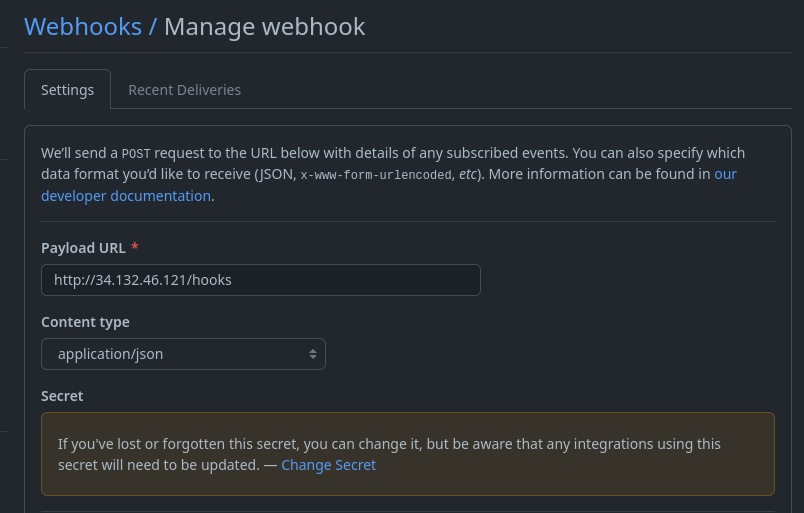
\includegraphics[width=12cm]{images/webhook1.png}
	\caption{Payload URL, Content type, and Webhook Secret.}
	\label{wh1}
\end{figure}
\vspace{2mm}


\begin{figure}[ht]
	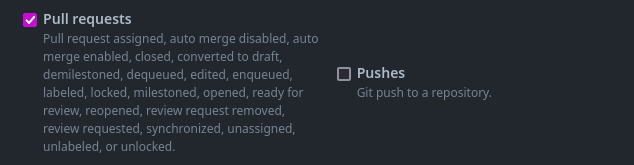
\includegraphics[width=12cm]{images/webhook2.png}
	\caption{Webhook trigger events.}
	\label{wh2}
\end{figure}
\vspace{2mm}

\subsection{\label{sec:gh_secrets}Github Secrets Configuration}

\justifying
The image in Figure \ref{gh_secrets} shows where to set the secrets in your Github repository. These should be named to match the values given in the GH action YAML file.
\vspace{2mm}

\begin{figure}[ht]
	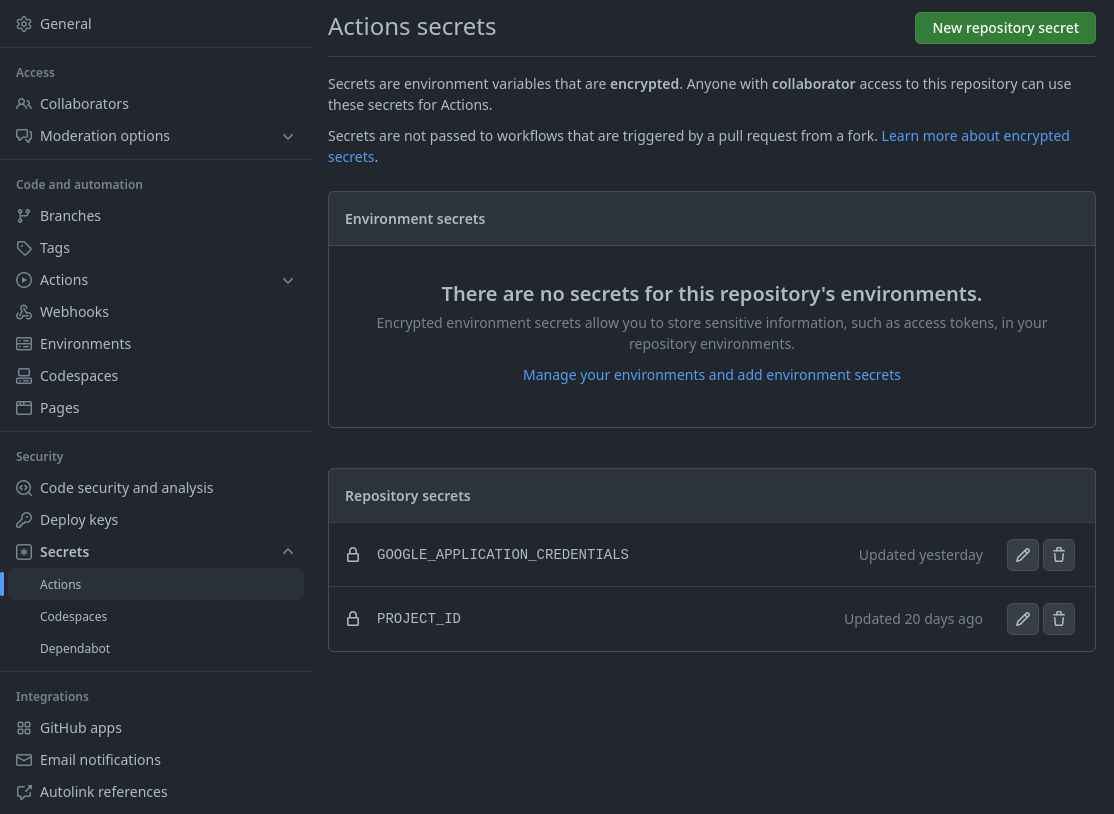
\includegraphics[width=12cm]{images/gh_secrets.png}
	\caption{Setting repository secrets.}
	\label{gh_secrets}
\end{figure}
\vspace{2mm}

\section{\label{sec:Python} The Python Application}

\justifying
The Python code is meant to run as a ``Cloud Function'' in GCP. This is a cost-effective way to run code becuase you can have
your application hosted without provisioning and maintaining any supporting infrastructure. We get to focus our code and let Google
take care of the rest.

\justifying
Our Python is reliant on a set of modules that are declared in the ``src/requirements.txt'' file.
\verbatiminput{../src/requirements.txt}

\justifying
There are a few other Python requirements files in the project that serve other purposes including testing and security.


\section{\label{sec:tf}Terraform}

\section{\label{sec:test}Testing}

\section{\label{sec:next}Going a Bit Further}

\justifying
This optional section describes how you can connect your Cloud Function to your Kubernetes cluster to extend the functionality even more.

\section{\label{sec:cleanup}Cleanup}

\justifying

docker system prune

\clearpage
\part{Appendix}

\appendix

\section{\label{sec:autotools}GNU Autotools}

\justifying
At the risk of introducing greater complexity, GNU Autotools have been included in the code base for the workshop. Autotools
are a well-maintained set of Open Source tools with a gentle learning curve and are included in the distribution of many Open
Source packages that we all rely on daily, at least indirectly, and often unknowingly. While it may be possible to complete this workshop
without at least learning how to configure and execute the tools in your environment, you will derive significantly less enjoyment
in doing so.
\vspace{2mm}

\justifying
The list of tools for using this Autotools configuration paradigm is show in Table \ref{Autotools}.
\vspace{2mm}

\begin{table}[ht]
	\centering
	\begin{tabular}{|l|l|}\hline
		Tool & Description \\\hline
		autoconf & Generates a configure script from configure.ac   \\\hline
		automake & Generates a system-specific Makefile based on Makefile.am template    \\\hline
		make  &   X    \\\hline
	\end{tabular}
	\caption{GNU tools used in this project}
	\label{Autotools}
\end{table}
\vspace{2mm}

\justifying
The image shown in Figure \ref{diagram} is from \cite{autobasics}.
It illustrates the relationship between components mentioned in Table \ref{Autotools}.
\vspace{2mm}

\begin{figure}[ht]
	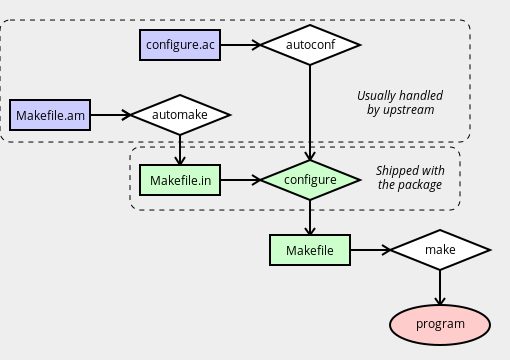
\includegraphics[width=12cm]{images/diagram.png}
	\caption{A basic overview of how the main Autotools components fit together.}
	\label{diagram}
\end{figure}
\vspace{2mm}


\clearpage
\begin{versionhistory}
	\vhEntry{v0.1}{October 2nd, 2022}{Franklin Diaz}{Initial Draft}
\end{versionhistory}

\clearpage
% \nocite{*}
\bibliographystyle{plain}
\bibliography{mybib}

\end{document}
